\clearpage
\section{Investigating Spinodal Decomposition in the Hf-Nb-Ti-V System}

The sections below apply the MLIP-informed pipeline---ORB potential energies, Jansson-based chemical potential derivatives, and a semi-implicit spectral Cahn--Hilliard solver---to the \ch{Hf-Nb-Ti-V} system.
We progress from binary to quaternary subsystems, demonstrating at each stage how thermodynamic driving forces, coherency strain, and numerical tractability jointly govern which compositions and temperatures are accessible to simulation.

Selecting a productive target composition requires meeting two criteria simultaneously.
The composition must be spinodally unstable ($\lambda_{\min} < 0$ for the Gibbs energy Hessian), and no individual element should exhibit a large positive diagonal Hessian entry $H_{ii} = \partial^2 G^\alpha_m / \partial x_i^2 \gg 0$ at the nominal composition.
Elements satisfying the latter condition are thermodynamically stable spectators: they do not drive decomposition, yet through the stability constraint on the semi-implicit spectral solver,
\begin{equation}
    \Delta t \;\leq\; \frac{C_{\rm s}\,\Delta x^{2}}{M\,H_{\max}},
    \label{eq:dt_stability}
\end{equation}
where $C_{\rm s} = 0.3$ is a safety factor, $\Delta x$ the grid spacing, $M$ the atomic mobility, and $H_{\max}$ the largest Hessian eigenvalue, they reduce the allowable time step by one to two orders of magnitude without contributing to any spinodal driving force (Supplementary Table~S1).
We address both criteria by studying the binary, ternary, and quaternary subsystems in sequence, selecting compositions and temperatures at which the spinodal is both thermodynamically strong and numerically tractable.

\subsection{Thermodynamic Stability Landscape}
\label{sec:stability_landscape}

The spinodal region of the BCC\textsubscript{A2} phase spans a wide but structured region of the Hf--Nb--Ti--V composition space whose extent and character change substantially with temperature.
Figure~\ref{fig:stability maps} shows affine projections of the number of negative eigenvalues of the chemical and coherent Gibbs energy Hessians at \qtylist{600;800;1000}{\kelvin}, computed at \SI{5}{\atpercent} sampling density in composition space.
Missing points represent convergence failures, most common at dilute compositions.
At \SI{600}{\kelvin}, coherent strain contributions most strongly suppress the chemical spinodal at compositions rich in Hf or V, and the region of two negative chemical eigenvalues vanishes entirely when coherency is included.
At \SI{800}{\kelvin}, the chemical Hessian predicts spinodal decomposition across nearly all compositions except those rich in Ti and Nb, while the coherent Hessian stabilizes solid solutions rich in both Hf and V.
At \SI{1000}{\kelvin}, coherent strain stabilizes all Ti- and V-rich compositions and the spinodal shrinks to a narrow Nb-rich band.

\begin{figure*}[!h]
        %\captionsetup[subfigure]{labelformat=empty}
        \centering
        \subfloat[(a)]{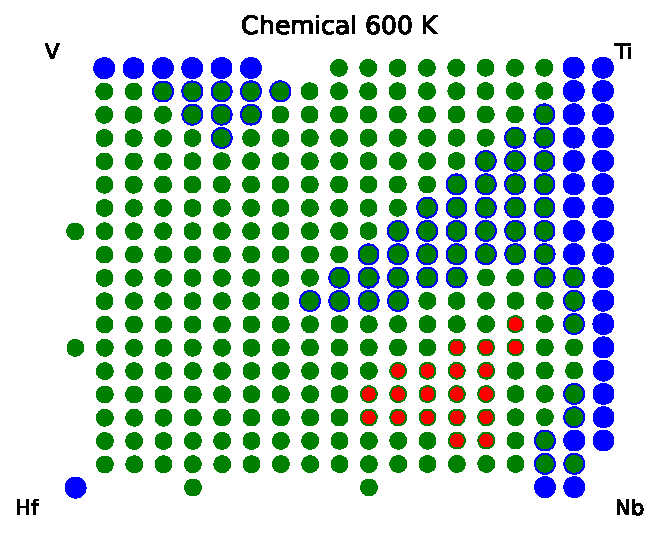
\includegraphics[width=.35\linewidth]{figs/chemical_600_diff_sizes.pdf}}\hspace{.3 in}
         \subfloat[(b)]{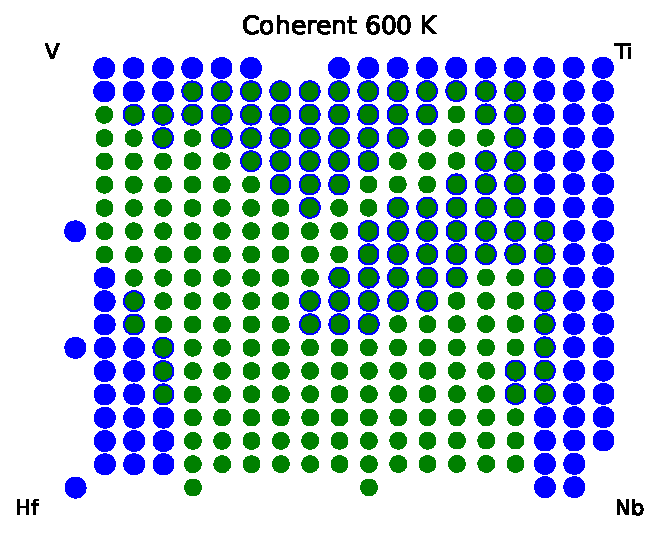
\includegraphics[width=.35\linewidth]{figs/coherent_600_diff_sizes.pdf}}\\
         \subfloat[(c)]{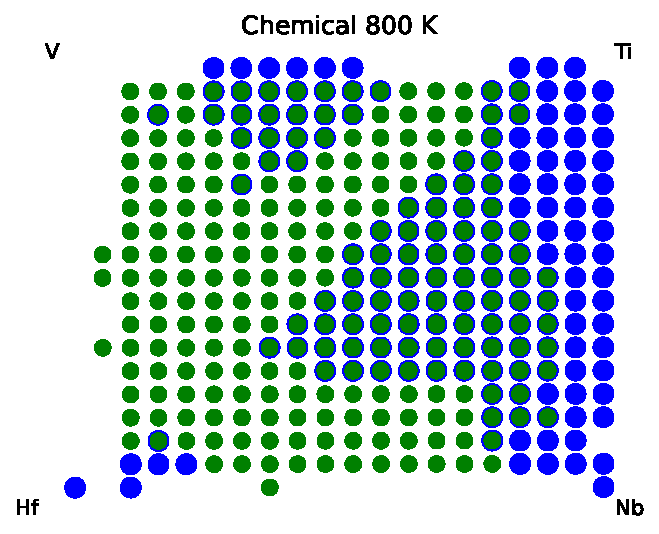
\includegraphics[width=.35\linewidth]{figs/chemical_800_diff_sizes.pdf}}\hspace{.3 in}
         \subfloat[(d)]{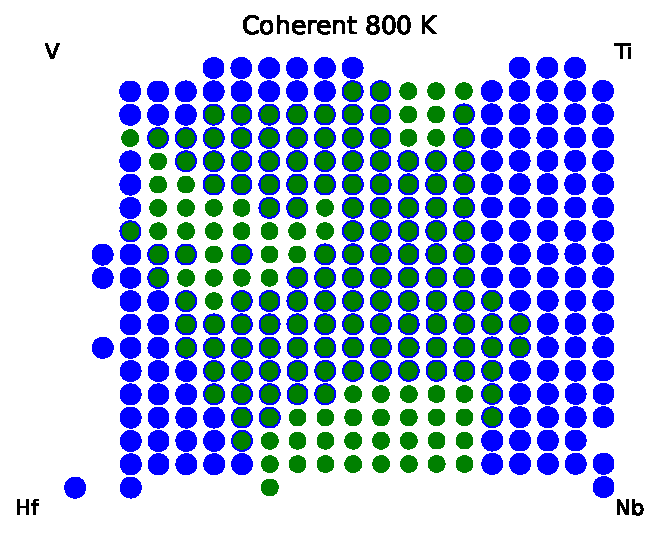
\includegraphics[width=.35\linewidth]{figs/coherent_800_diff_sizes.pdf}}\\
         \subfloat[(e)]{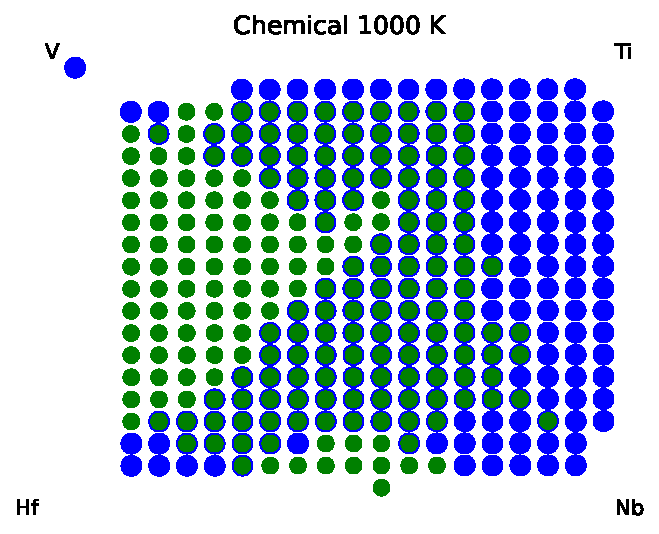
\includegraphics[width=.35\linewidth]{figs/chemical_1000_diff_sizes.pdf}}\hspace{.3 in}
         \subfloat[(f)]{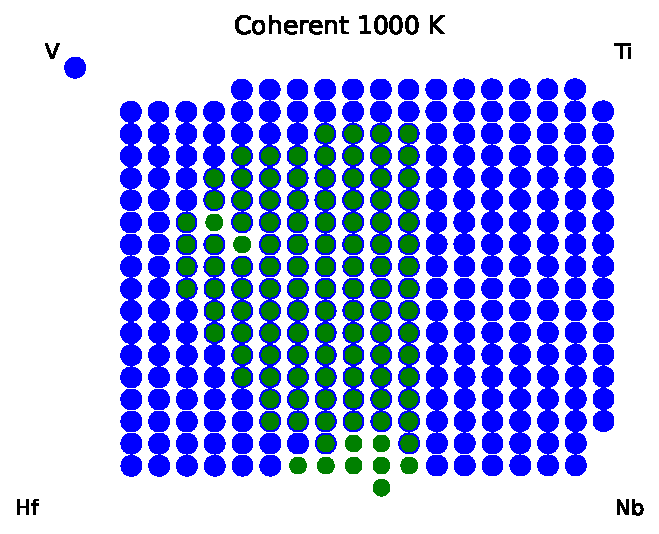
\includegraphics[width=.35\linewidth]{figs/coherent_1000_diff_sizes.pdf}}\\
         \subfloat[]
         {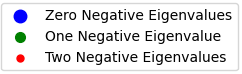
\includegraphics[width=.3\linewidth]{figs/legend.png}}
         \caption{Affine projection stability maps displaying the number of negative eigenvalues of the chemical and coherent Gibbs energy Hessian for BCC\textsubscript{A2} in the \ch{Hf-Nb-Ti-V} system at (a,b)~\SI{600}{\kelvin}, (c,d)~\SI{800}{\kelvin}, and (e,f)~\SI{1000}{\kelvin}.
         Left column: chemical Hessian; right column: coherent Hessian.
         Coherent strain suppresses the spinodal most strongly in Hf- and V-rich compositions across all temperatures.}
\label{fig:stability maps}
\end{figure*}

The mechanism by which coherency suppresses the Hf-rich spinodal is revealed by the first eigenvector of the chemical Hessian.
Figure~\ref{fig:eigenvector} shows the components of this vector for BCC \ch{Hf_{0.6}Nb_{0.1}Ti_{0.1}V_{0.2}} from \qtyrange{600}{1000}{\kelvin}, a composition at which the chemical Hessian is negative while all eigenvalues of the coherent Hessian are positive.
The unstable fluctuation mode corresponds to enrichment in Hf at the expense of V.
Since Hf and V have the largest atomic radius mismatch of the four constituents, this fluctuation mode incurs the greatest coherency penalty: adding the elastic contribution to the Gibbs energy reverses the sign of the local curvature and stabilizes the alloy against this mode throughout the temperature range shown.
The element pair that drives the chemical instability is self-suppressed by the strain energy it would generate.

\begin{figure*}[!h]
\centering
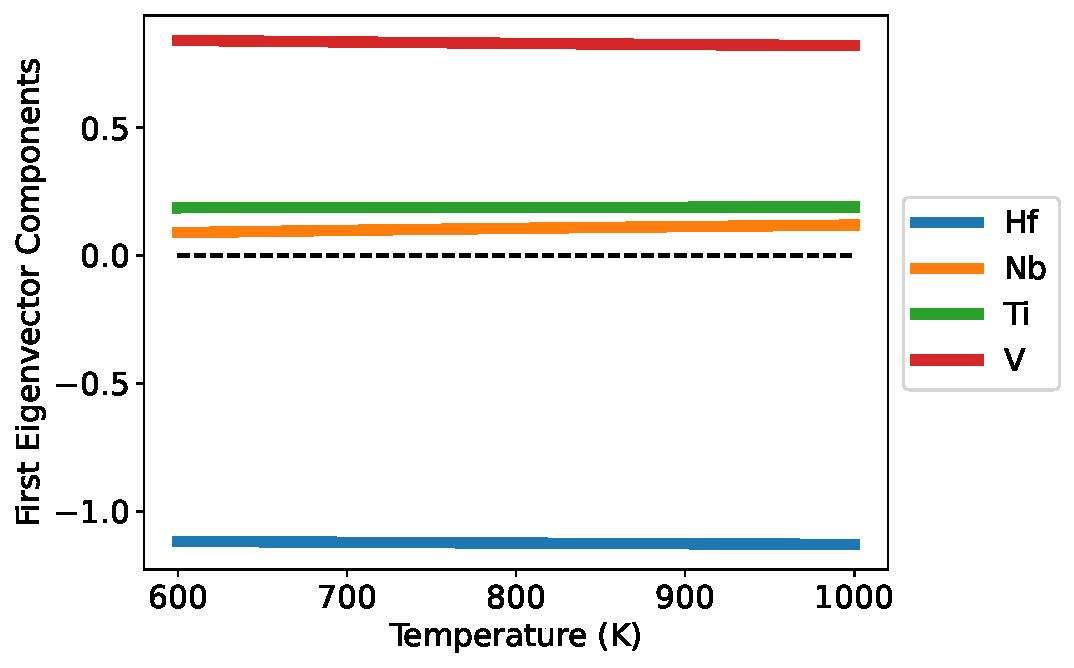
\includegraphics[width=\linewidth]{figs/eigenvector.pdf}
\caption{Components of the first gauge-invariant eigenvector of the chemical Hessian as a function of temperature for BCC \ch{Hf_{0.6}Nb_{0.1}Ti_{0.1}V_{0.2}}.
The dominant instability mode corresponds to Hf-enrichment at the expense of V; the large Hf--V atomic radius mismatch causes coherent strain to stabilize this mode at all temperatures shown, reversing the sign of the first eigenvalue from negative (chemical) to positive (coherent).}
\label{fig:eigenvector}
\end{figure*}

The temperature at which spinodal decomposition becomes accessible is composition-dependent and shifts substantially when coherency is included (Fig.~\ref{fig:eigenvalues}).
For the Ti- and Nb-rich composition \ch{Hf_{0.10}Nb_{0.40}Ti_{0.40}V_{0.10}}, the chemical and coherent spinodal temperatures are nearly identical, reflecting the small misfit penalty in dilute-Hf alloys.
For the equiatomic composition \ch{Hf_{0.25}Nb_{0.25}Ti_{0.25}V_{0.25}}, both Hessians become negative below ${\sim}\SI{800}{\kelvin}$, confirming that this alloy is coherently spinodal at \SI{500}{\celsius}, the temperature adopted for all phase-field simulations below.
For the Hf-rich composition \ch{Hf_{0.6}Nb_{0.1}Ti_{0.1}V_{0.2}}, the coherent Hessian remains positive at all temperatures shown, consistent with the eigenvector analysis above.

\begin{figure*}[!h]
        %\captionsetup[subfigure]{labelformat=empty}
        \centering
        \subfloat[(a)]{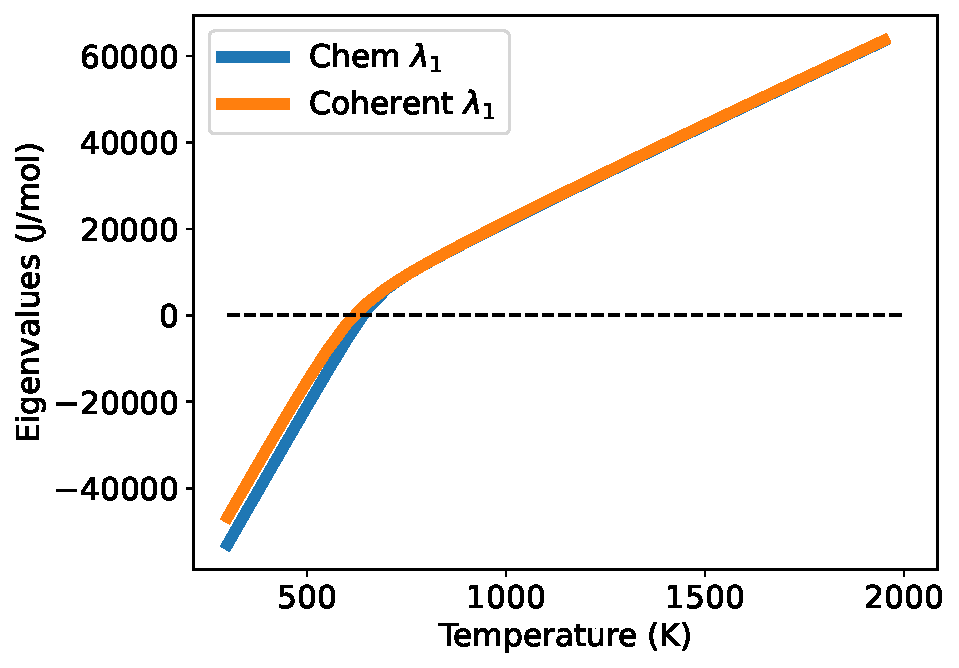
\includegraphics[width=.35\linewidth]{figs/eigenvalues_Hf1.pdf}}\hspace{.3 in}
         \subfloat[(b)]{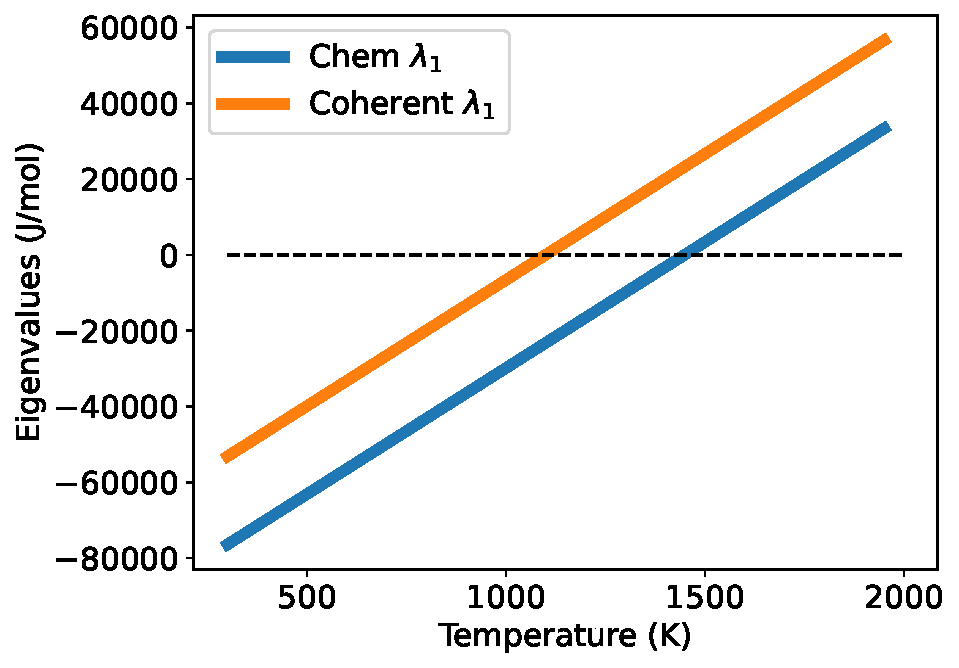
\includegraphics[width=.35\linewidth]{figs/eigenvalues_Hf25.pdf}}\\
         \subfloat[(c)]{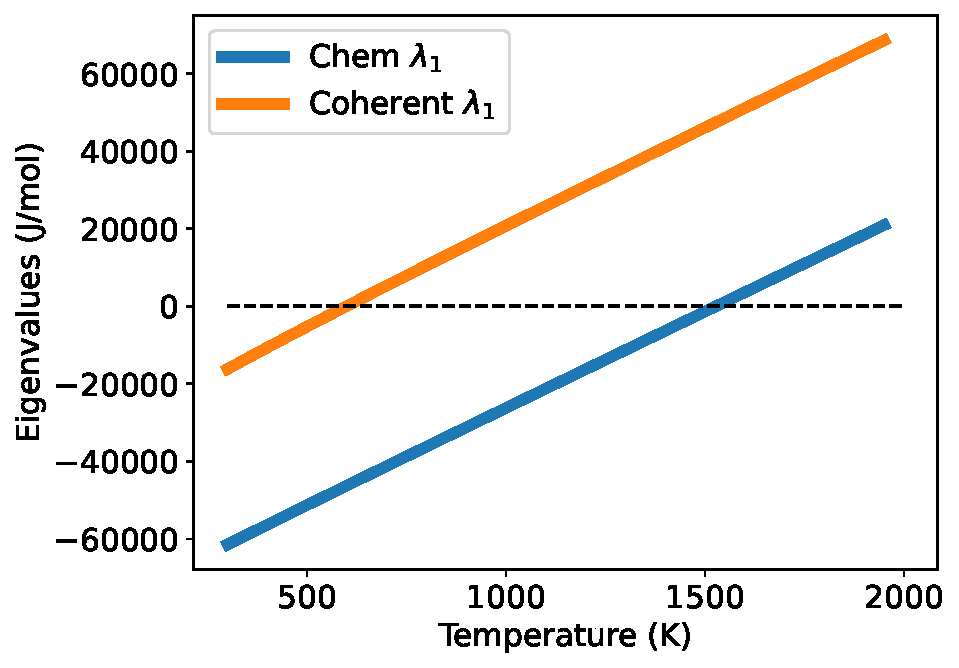
\includegraphics[width=.35\linewidth]{figs/eigenvalues_Hf4.pdf}}
         \caption{Gauge-invariant first eigenvalue of the chemical and coherent Gibbs energy Hessian as a function of temperature for BCC (a)~\ch{Hf_{0.10}Nb_{0.40}Ti_{0.40}V_{0.10}}, (b)~\ch{Hf_{0.25}Nb_{0.25}Ti_{0.25}V_{0.25}}, and (c)~\ch{Hf_{0.6}Nb_{0.1}Ti_{0.1}V_{0.2}}.
         Coherency shifts the spinodal temperature downward most strongly in Hf-rich alloys.
         The equiatomic composition (b) is coherently spinodal below ${\sim}\SI{800}{\kelvin}$, confirming \SI{500}{\celsius} as a tractable simulation temperature.}
\label{fig:eigenvalues}
\end{figure*}

\clearpage

\subsection{Binary Nb--V: First Demonstration of the MLIP-Informed Pipeline}
\label{sec:binary}

The binary Nb--V system is the first demonstration of the complete framework: a machine-learned interatomic potential (ORB) supplies the thermodynamic database, Jansson interpolation evaluates chemical potentials and their composition derivatives directly from the CALPHAD dataset --- bypassing finite-difference approximations --- and the spectral Cahn-Hilliard solver propagates the resulting elasto-chemical driving forces on the grid.
The single independent composition field isolates the Jansson derivative from multi-component complexity, and the well-characterized miscibility gap at \SI{500}{\celsius} with no spectator elements provides a clean validation setting before extension to the ternary and quaternary subsystems.
The equilibrium BCC\textsubscript{A2} tie-line endpoints at \SI{500}{\celsius} are an Nb-rich phase ($x_{\rm Nb} = 0.96$) and a V-rich phase ($x_{\rm Nb} = 0.36$), between which the stiffness tensors $C_{ij}$ and Vegard eigenstrain coefficient $\alpha_{\rm Nb} = \partial\ln a/\partial x_{\rm Nb}$ are linearly interpolated from SQS configurations evaluated with the ORB machine-learned interatomic potential.
The coefficient $\alpha_{\rm Nb} = 0.0874$ is evaluated at the tie-line midpoint ($x_{\rm Nb} = 0.66$, $a_{\rm ref} = \SI{3.228}{\angstrom}$), giving a total misfit strain $\varepsilon_T = -5.5\%$ between the two equilibrium phases and a molar volume $N_V = \SI{8.99e4}{\mol\per\metre\cubed}$.
Table~\ref{tab:binary_elastic} lists the full elastic constants and derived properties at both endpoints.

\begin{table}[!h]
    \centering
    \caption{%
        Elastic constants and Vegard eigenstrain parameters for the Nb--V
        BCC\textsubscript{A2} tie-line endpoints at \SI{500}{\celsius},
        computed from SQS configurations evaluated with the ORB
        machine-learned interatomic potential.
        $C' = (C_{11}-C_{12})/2$: tetragonal shear modulus;
        $A_Z = C_{44}/C'$: Zener anisotropy ratio;
        $\varepsilon_T = (a_{\rm ppt} - a_{\rm mat})/a_{\rm mat}$: misfit strain.
    }
    \label{tab:binary_elastic}
    \renewcommand{\arraystretch}{0.8}
    \setlength{\tabcolsep}{5pt}
    \begin{tabular}{lcc}
        \toprule
        Property & Nb-rich ($x_{\rm Nb}=0.96$) & V-rich ($x_{\rm Nb}=0.36$) \\
        \midrule
        \multicolumn{3}{l}{\textit{Composition and lattice parameter}} \\
        $x_{\rm Nb}$ & 0.96 & 0.36 \\
        $x_{\rm V}$  & 0.04 & 0.64 \\
        $a$ (\AA)    & 3.312 & 3.130 \\
        \midrule
        \multicolumn{3}{l}{\textit{Cubic elastic constants (GPa)}} \\
        $C_{11}$ & 243.6 & 259.3 \\
        $C_{12}$ & 119.7 & 145.0 \\
        $C_{44}$ &  20.6 &  18.0 \\
        $C' = (C_{11}-C_{12})/2$ & 62.0 & 57.2 \\
        \midrule
        \multicolumn{3}{l}{\textit{Derived elastic properties}} \\
        $G_{\rm VRH}$ (GPa) & 32.5 & 29.2 \\
        $B_{\rm VRH}$ (GPa) & 161.0 & 183.1 \\
        Poisson ratio $\nu$ & 0.406 & 0.424 \\
        Zener ratio $A_Z = C_{44}/C'$ & \textbf{0.332} & \textbf{0.315} \\
        \midrule
        \multicolumn{3}{l}{\textit{Vegard eigenstrain parameters (shared)}} \\
        $a_{\rm ref}$ (\AA) & \multicolumn{2}{c}{3.228} \\
        $\alpha_{\rm Nb} = \partial\ln a/\partial x_{\rm Nb}$ & \multicolumn{2}{c}{0.0874} \\
        $\varepsilon_T = \Delta a / a_{\rm mat}$ & \multicolumn{2}{c}{$-5.5\%$} \\
        $N_V$ (mol\,m$^{-3}$) & \multicolumn{2}{c}{$8.99\times10^{4}$} \\
        \bottomrule
    \end{tabular}
\end{table}

Both endpoints have $A_Z < 1$ (\Cref{tab:binary_elastic}), identifying $\langle 110 \rangle$ as the elastically soft direction.
Figure~\ref{fig:chem_vs_elastic} shows the output of the MLIP-informed pipeline across four mean compositions.
The chemical-only simulations (top row) produce isotropic interconnected domains at all four compositions, with no preferred orientation.
The elasto-chemical simulations (bottom row) reveal a composition-dependent response that is absent in the chemical-only case.
At $x_{\rm Nb}^0 = 0.50$, coherency strain completely suppresses spinodal decomposition and the field remains uniform, consistent with the coherent Hessian analysis showing that elastic energy closes the miscibility gap at the symmetric composition.
At $x_{\rm Nb}^0 = 0.60$ and $0.70$, decomposition proceeds and produces a labyrinthine, bicontinuous morphology with channels preferentially aligned along $\langle 110 \rangle$, reflecting the elastically soft direction ($A_Z < 1$).
At $x_{\rm Nb}^0 = 0.80$, the V-rich phase constitutes a small minority and forms isolated $\langle 110 \rangle$-elongated islands embedded in a continuous Nb-rich matrix.

The absence of decomposition at $x_{\rm Nb}^0 = 0.50$ reflects a direct thermodynamic consequence of coherency: at this composition and temperature, the elastic penalty is sufficient to render the smallest positive eigenvalue of the coherent Gibbs energy Hessian positive, stabilizing the alloy against all composition fluctuations. That the chemical-only simulation at the same composition decomposes freely establishes that this stability is entirely elastic in origin. Coherency strain thus closes the miscibility gap at the symmetric composition in Nb--V --- an effect that a purely chemical phase-field model would miss entirely.

\begin{figure}[!h]
    \centering
    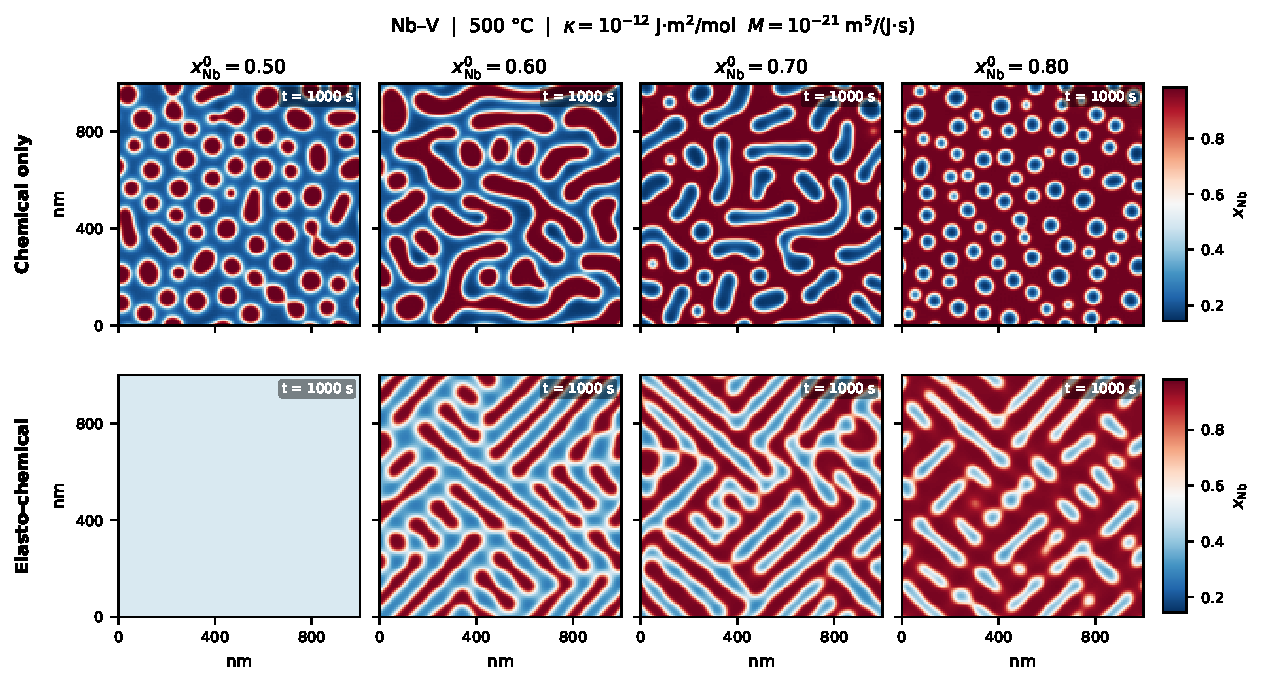
\includegraphics[width=\textwidth]{figs/chem_vs_elastic_final.pdf}
    \caption{%
        Simulated $x_{\rm Nb}$ microstructures from Cahn-Hilliard
        simulations of binary Nb--V BCC\textsubscript{A2} at
        \SI{500}{\celsius} ($128\times128$ grid,
        $L = \SI{1}{\micro\metre}$,
        $\kappa = \SI{1e-12}{\joule\metre\squared\per\mol}$,
        $M = \SI{5e-21}{\metre\tothe{5}\per\joule\per\second}$).
        Top row: chemical only.
        Bottom row: elasto-chemical (tensorial Vegard coupling,
        $\alpha_{\rm Nb} = 0.087$, cubic stiffness from SQS/DFT).
        Columns correspond to mean compositions
        $x_{\rm Nb}^0 = 0.50,\,0.60,\,0.70,\,0.80$.
        Colormap: $x_{\rm Nb}$ increases from blue (low) to red (high).
        Both phases have $A_Z < 1$, selecting $\langle 110 \rangle$-aligned
        boundaries and the characteristic diamond-faceted morphology in the
        elasto-chemical case.
    }
    \label{fig:chem_vs_elastic}
\end{figure}

\subsection{Ternary Nb--Hf--V: Temperature and Composition Dependence}
\label{sec:ternary}

Adding Hf to the binary Nb--V system changes the character of the spinodal instability qualitatively.
Table~\ref{tab:spinodal_regimes} summarizes four distinct regimes for the ternary Nb$_{50}$Hf$_5$V$_{45}$ alloy across \SIrange{500}{1000}{\celsius}, identified from the signs of the diagonal Hessian elements $H_{\rm Nb}$, $H_{\rm Hf}$, and $H_{\rm V} = H_{\rm Nb} + H_{\rm Hf} + 2H_{\rm Nb,Hf}$.
Above \SI{700}{\celsius}, no diagonal instability exists; the spinodal is driven solely by weak off-diagonal Nb--Hf coupling ($\lambda_{\min} \lesssim 0$) and produces no significant decomposition.
Between \SI{600}{\celsius} and \SI{700}{\celsius}, only $H_{\rm Nb} < 0$: Nb segregates asymmetrically against a stable V$+$Hf background, with Hf acting as an inert spectator.
Below \SI{500}{\celsius}, $H_{\rm V}$ also turns negative, recovering a binary-like Nb--V demixing, but Hf remains a positive-curvature stiffener that suppresses $\Delta t$.
The most numerically tractable temperature for this ternary is \SI{700}{\celsius}, where the Nb-driven spinodal ($|\lambda_{\min}| = \SI{13272}{\joule\per\mol}$) is active without the stiffness penalty, albeit with a driving force approximately six times weaker than at \SI{500}{\celsius}.

\begin{table}[!h]
    \centering
    \caption{%
        Spinodal character and equilibrium two-phase compositions as a function
        of temperature for the binary Nb$_{50}$V$_{50}$ and ternary
        Nb$_{50}$Hf$_5$V$_{45}$ BCC\textsubscript{A2} alloys.
        Signs of the diagonal Hessian elements indicate whether each element
        is individually unstable ($H_{ii} < 0$, driving force) or stable
        ($H_{ii} > 0$, spectator).
        $H_{\rm V}$ is derived via
        $H_{\rm V} = H_{\rm Nb} + H_{\rm Hf} + 2H_{\rm Nb,Hf}$.
    }
    \label{tab:spinodal_regimes}
    \scriptsize
    \renewcommand{\arraystretch}{1.0}
    \begin{tabularx}{\textwidth}{lllll}
        \toprule
        Regime & System & Diagonal instabilities & Physical character & Equilibrium BCC phases$^{a}$ \\
        \midrule
        $T < \SI{750}{\celsius}$
            & Binary Nb$_{50}$V$_{50}$
            & $H_{\rm Nb} = H_{\rm V} < 0$
            & Symmetric Nb$\leftrightarrow$V demixing; both components drive decomposition equally
            & BCC$_1$: Nb$_{99}$V$_{1}$\newline BCC$_2$: Nb$_{1}$V$_{99}$ \\
        $T > \SI{700}{\celsius}$
            & Ternary Nb$_{50}$Hf$_5$V$_{45}$
            & None ($H_{\rm Nb},\,H_{\rm Hf},\,H_{\rm V} > 0$)
            & No diagonal instability; only weak off-diagonal Nb--Hf coupling drives marginal spinodal ($\lambda_{\min} \lesssim 0$); no significant decomposition
            & Single-phase BCC: Nb$_{50}$Hf$_{5}$V$_{45}$ \\
        \SIrange{600}{700}{\celsius}
            & Ternary Nb$_{50}$Hf$_5$V$_{45}$
            & $H_{\rm Nb} < 0$ only
            & Asymmetric spinodal: Nb segregates against a stable V$+$Hf matrix; Hf acts as inert spectator
            & BCC$_1$: Nb$_{90}$Hf$_{9}$V$_{1}$\newline BCC$_2$: Nb$_{2}$Hf$_{0.1}$V$_{98}$ \\
        $T < \SI{500}{\celsius}$
            & Ternary Nb$_{50}$Hf$_5$V$_{45}$
            & $H_{\rm Nb} < 0$,\; $H_{\rm V} < 0$
            & Binary-like Nb--V demixing; Hf remains stable ($H_{\rm Hf} > 0$) and imposes numerical stiffness
            & BCC$_1$: Nb$_{91}$Hf$_{9}$V$_{0.3}$\newline BCC$_2$: Nb$_{0.6}$Hf$_{0.04}$V$_{99}$ \\
        \bottomrule
        \multicolumn{5}{l}{\footnotesize $^{a}$~Equilibrium tie-line endpoints computed with \texttt{pycalphad}
            (\texttt{BCC\_A2} miscibility gap) using an ORB-MLIP CALPHAD database for the HfNbTiV system.
            Subscripts are at.\%; representative temperatures: \SI{500}{\celsius} for
            $T<\SI{750}{\celsius}$ rows, \SI{700}{\celsius} for the
            \SIrange{600}{700}{\celsius} row.}
    \end{tabularx}
\end{table}

Figure~\ref{fig:ternary_summary} consolidates three further perspectives on the ternary system.
The Hf sweep (panels a--e) shows that at low Hf fractions ($x_{\rm Hf}^0 = 0.05$, 0.10) decomposition produces isolated Nb-rich precipitates consistent with a minority-phase microstructure; increasing Hf to 0.20 and 0.25 shifts the tie-line endpoints and produces well-developed bicontinuous Nb--V domains, indicating that Hf progressively deepens the miscibility gap.
The middle row (panels e--f) isolates the elastic contribution at $x_{\rm Hf}^0 = 0.25$: the chemical-only simulation (e) produces isotropic interconnected domains, while the elasto-chemical case (f) remains nearly uniform, demonstrating that coherency strain again closes the miscibility gap at this composition, extending the suppression seen in the binary at $x_{\rm Nb}^0 = 0.50$ to the ternary.
The bottom row (panels g--h) shows the temperature dependence for Nb$_{50}$Hf$_5$V$_{45}$: at \SI{500}{\celsius} (g) decomposition is early-stage with small, diffuse Nb-rich clusters, while at \SI{600}{\celsius} (h) the domains are better developed despite the higher temperature, consistent with the Hessian analysis showing that $H_{\rm Nb} < 0$ with a moderate driving force at \SI{600}{\celsius} while the system sits closer to the spinodal boundary at \SI{500}{\celsius} for this dilute-Hf composition.
Panel (i) places these simulations in context by showing the ternary BCC\textsubscript{A2} miscibility gap across all three binary subsystems (Hf--Nb, Nb--V, Hf--V), with the composition space accessible to the ternary highlighted.

\begin{figure*}[!h]
    \centering
    \begin{overpic}[width=\textwidth]{figs/hf_sweep}
    \put(0, 20){\textbf{(a)}}
    \end{overpic}
    %%%
    \begin{overpic}[width=\textwidth]{figs/hf_sweep_elastic}
    \put(0, 20){\textbf{(b)}}
    \end{overpic}
    %%%
    \begin{overpic}[width=0.6\textwidth]{figs/Spinodal Ternary Phase Diagram Figure.png}
    \put(0, 80){\textbf{(c)}}
    \end{overpic}
    \caption{%
        Hf-content sweep of $x_{\rm Nb}$ microstructures in ternary
        Nb--Hf--V BCC\textsubscript{A2} at \SI{500}{\celsius}
        ($128\times128$ grid, $L = \SI{1}{\micro\metre}$,
        $\kappa = \SI{1e-12}{\joule\metre\squared\per\mol}$,
        $M_{\rm Nb} = \SI{5e-21}{\metre\tothe{5}\per\joule\per\second}$).
        \textbf{(a)} Chemical-only simulations.
        \textbf{(b)} Elasto-chemical simulations with Vegard coherency strain;
        panels marked ``simulation pending'' are reserved for calculations in
        progress.
        \textbf{(c)} Ternary BCC\textsubscript{A2} miscibility gap across all
        three binary subsystems (Hf--Nb, Nb--V, Hf--V).
        Colormap: $x_{\rm Nb}$ increases from blue (low) to red (high).
    }
    \label{fig:ternary_summary}
\end{figure*}

\subsection{Quaternary HfNbTiV: Phase-Field Prediction and Experimental Validation}
\label{sec:quaternary}

\subsubsection{Chemical-only microstructure and CALPHAD tie-line}

The equiatomic composition Nb$_{25}$Hf$_{25}$Ti$_{25}$V$_{25}$ satisfies both criteria identified in Section~\ref{sec:stability_landscape}: $\lambda_{\min} < 0$ at \SI{500}{\celsius} and, with the mobility assignments described below, sufficient microstructural evolution is accessible within $10^6$ steps.
Figure~\ref{fig:quaternary_chem} shows the composition fields from a chemical-only Cahn-Hilliard simulation ($128\times128$ grid, $L = \SI{1}{\micro\metre}$, $\Delta t = \SI{0.1}{\second}$, $\boldsymbol{\kappa} = [\num{1e-12},\,\num{7e-12},\,\num{1e-12}]\,\si{\joule\metre\squared\per\mol}$, $\mathbf{M} = \operatorname{diag}[\num{5e-21},\,\num{5e-23},\,\num{5e-21}]\,\si{\metre\tothe{5}\per\joule\per\second}$) at step 600{,}000.
Ellipsoidal V-rich precipitates form in an Nb/Hf/Ti-rich matrix; the diffuse Hf halos around precipitate cores reflect the tenfold lower Hf mobility relative to Nb and Ti rather than an independent Hf instability.

To validate the partitioning directions and obtain physically correct tie-line endpoints for the elasto-chemical simulation, we computed the CALPHAD equilibrium tie-line at \SI{500}{\celsius} using \texttt{pycalphad} with an ORB-MLIP CALPHAD database for the HfNbTiV system (\Cref{tab:quaternary_tieline}).
Two BCC\textsubscript{A2} phases coexist: an Nb/Hf/Ti-rich matrix (phase fraction $\approx 0.67$) and a V-rich precipitate (phase fraction $\approx 0.33$).
The phase-field partitioning directions match the CALPHAD prediction for all four elements; Nb and V compositions agree quantitatively, while Hf and Ti have not yet reached their equilibrium values at step 600{,}000, consistent with slow Hf kinetics and residual V in the matrix.

\begin{table}[!h]
    \centering
    \caption{%
        CALPHAD equilibrium tie-line endpoints for equiatomic
        Nb$_{25}$Hf$_{25}$Ti$_{25}$V$_{25}$ BCC\textsubscript{A2} at
        \SI{500}{\celsius}, computed with \texttt{pycalphad} using the
        ORB-MLIP CALPHAD database for the HfNbTiV system.
        Phase-field composition ranges from the final frame (step 600{,}000)
        are shown for comparison; PFM values are non-equilibrium, particularly
        for Hf (slow kinetics) and V (matrix still draining).
    }
    \label{tab:quaternary_tieline}
    \renewcommand{\arraystretch}{1.3}
    \setlength{\tabcolsep}{5pt}
    \begin{tabular}{llcccc}
        \toprule
        & & $x_{\rm Nb}$ & $x_{\rm Hf}$ & $x_{\rm Ti}$ & $x_{\rm V}$ \\
        \midrule
        \multirow{2}{*}{CALPHAD tie-line}
            & Matrix ($f \approx 0.67$)
            & 0.300 & 0.371 & 0.305 & 0.024 \\
            & Precipitate ($f \approx 0.33$)
            & 0.148 & 0.002 & 0.136 & 0.714 \\
        \midrule
        \multirow{2}{*}{PFM (step 600{,}000)}
            & Matrix
            & $\approx 0.30$ & $\approx 0.33$ & $\approx 0.29$ & $\approx 0.11$ \\
            & Precipitate
            & $\approx 0.11$ & $\approx 0.06$ & $\approx 0.06$ & $\approx 0.68$ \\
        \bottomrule
    \end{tabular}
\end{table}

\begin{figure}[!h]
    \centering
    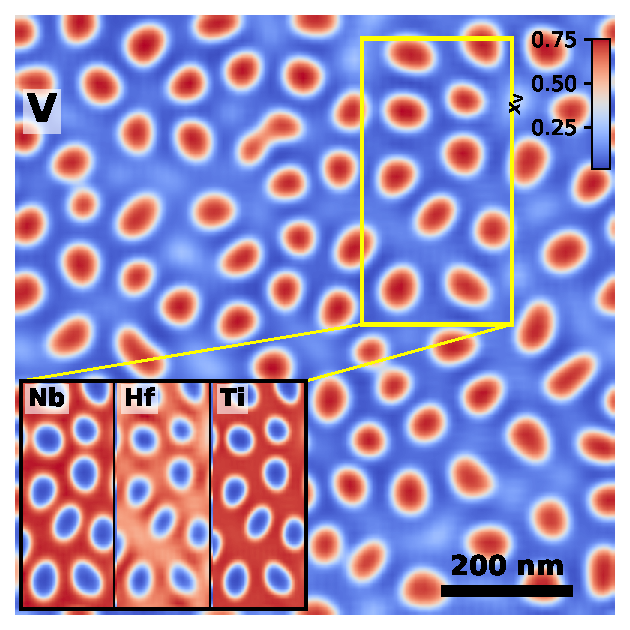
\includegraphics[width=\textwidth]{figs/quaternary_chem_step600k.pdf}
    \caption{%
        Composition fields from the chemical-only Cahn-Hilliard simulation of
        equiatomic Nb$_{25}$Hf$_{25}$Ti$_{25}$V$_{25}$ BCC\textsubscript{A2}
        at \SI{500}{\celsius} ($128\times128$ grid, $L = \SI{1}{\micro\metre}$,
        step 600{,}000, $\Delta t = \SI{0.1}{\second}$).
        From left to right: $x_{\rm Nb}$, $x_{\rm Hf}$, $x_{\rm Ti}$, $x_{\rm V}$.
        V-rich precipitates (blue in $x_{\rm Nb}$, $x_{\rm Hf}$, $x_{\rm Ti}$;
        red in $x_{\rm V}$) are embedded in an Nb/Hf/Ti-rich matrix.
        Diffuse halos in $x_{\rm Hf}$ reflect the tenfold lower Hf mobility
        ($M_{\rm Hf} = \SI{5e-23}{\metre\tothe{5}\per\joule\per\second}$).
        Partitioning directions are consistent with the CALPHAD tie-line
        (\Cref{tab:quaternary_tieline}).
    }
    \label{fig:quaternary_chem}
\end{figure}

\subsubsection{Elasto-chemical prediction and comparison with experiment}

The elastic response of the quaternary system differs fundamentally from the binary baseline of Section~\ref{sec:binary}.
At the CALPHAD tie-line matrix composition, the SQS/DFT interpolant yields $A_Z^{\rm mat} = 1.52 > 1$, identifying $\langle 100 \rangle$ as the elastically soft direction — the opposite selection from the binary NbV case ($A_Z = 0.33 < 1$).
Table~\ref{tab:elastic_comparison} compares the full set of model predictions against the experimental characterization of equiatomic HfNbTiV by An~et~al.\ \cite{an2021spinodal}, who identified two coexisting BCC\textsubscript{A2} phases in an as-cast alloy by XRD, HAADF-STEM, and EDS.

\begin{table}[!h]
    \centering
    \caption{%
        Predicted and experimentally measured properties for the equiatomic
        BCC\textsubscript{A2} HfNbTiV alloy.
        Experimental values are from An~et~al.\ \cite{an2021spinodal} (as-cast,
        characterized by XRD, HAADF-STEM, and EDS).
        Binary predictions use the NbV tie-line endpoints; quaternary
        predictions use the CALPHAD tie-line at \SI{500}{\celsius}
        (\Cref{tab:quaternary_tieline}).
        $A_Z = 2C_{44}/(C_{11}-C_{12})$: $A_Z > 1$ selects
        $\langle 100 \rangle$ modulation, $A_Z < 1$ selects
        $\langle 110 \rangle$.
        $\varepsilon_T = (a_{\rm ppt} - a_{\rm mat})/a_{\rm mat}$.
    }
    \label{tab:elastic_comparison}
    \renewcommand{\arraystretch}{1.3}
    \setlength{\tabcolsep}{4pt}
    \begin{tabularx}{\textwidth}{lXXX}
        \toprule
        Property
            & Experiment \cite{an2021spinodal}
            & Binary NbV (this work)
            & Quaternary NbHfTiV (this work) \\
        \midrule
        Precipitate enriched in
            & Hf $+$ V
            & V
            & V (Hf in matrix) \\
        Matrix enriched in
            & Nb $+$ Ti
            & Nb
            & Nb, Hf, Ti \\
        Precipitate phase fraction
            & $\approx 1/3$
            & ---
            & $\approx 0.33$ \\
        $a_{\rm mat}$ (\AA)
            & 3.313
            & 3.312
            & 3.382 \\
        $a_{\rm ppt}$ (\AA)
            & 3.259
            & 3.130
            & 3.089 \\
        $\varepsilon_T$
            & $-1.6\%$ (XRD); $0.54\%$ (TEM)
            & $-5.5\%$
            & $-8.7\%$ \\
        $A_Z$ (matrix)
            & ---
            & 0.33
            & \textbf{1.52} \\
        $A_Z$ (precipitate)
            & ---
            & 0.31
            & 0.32 \\
        Spinodal modulation direction
            & $\langle 100 \rangle$
            & $\langle 110 \rangle$ (predicted)
            & $\langle 100 \rangle$ (predicted) \\
        Modulation wavelength
            & ${\approx}\SI{50}{\nano\metre}$
            & ---
            & ${\approx}50$--\SI{100}{\nano\metre} \\
        \bottomrule
    \end{tabularx}
\end{table}

Three findings emerge from this comparison.

\textit{Hf partitioning is inconsistent between the CALPHAD model and experiment.}
An~et~al.\ demonstrate via HAADF-STEM Z-contrast that Hf ($Z = 72$, the heaviest constituent) enriches the precipitate phase ($\beta^*$), co-segregating with V.
The ORB-MLIP CALPHAD model assigns Hf to the matrix alongside Nb and Ti (\Cref{tab:quaternary_tieline}).
The most likely origin of this discrepancy is the thermal history: the experimental alloy was drop-cast and spinodal decomposition occurred during rapid cooling from the melt, far from the \SI{500}{\celsius} equilibrium tie-line used in the simulation.
Non-equilibrium partitioning during rapid quenching can favor kinetically accessible configurations that differ from the thermodynamic ground state, particularly for a heavy element such as Hf whose equilibrium diffusivity is low.

\textit{The misfit strain is overestimated by the CALPHAD model.}
An~et~al.\ report a lattice misfit of $-1.6\%$ from XRD peak separation and $0.54\%$ from TEM atomic-column measurements, both substantially smaller than the $-8.7\%$ predicted by the quaternary CALPHAD tie-line.
This overestimate is a direct consequence of the incorrect Hf partitioning: if Hf (large atomic radius, $a_{\rm Hf}^{\rm BCC} \approx \SI{3.62}{\angstrom}$) were to co-enrich the precipitate with V (small atomic radius, $a_{\rm V}^{\rm BCC} \approx \SI{3.03}{\angstrom}$), the opposing contributions to the precipitate lattice parameter would partially cancel, yielding a much smaller net misfit consistent with experiment.
The binary NbV misfit of $-5.5\%$ is also larger than the experimental value, though less severely so.

\textit{The quaternary elastic anisotropy correctly predicts the observed spinodal modulation direction.}
The HAADF-STEM fast Fourier transform patterns in An~et~al.\ (Fig.~1(e,f) of that work) show spinodal modulation wavevectors along $\langle 100 \rangle$, the elastically soft direction for alloys with $A_Z > 1$.
The quaternary CALPHAD model gives $A_Z^{\rm mat} = 1.52 > 1$ for the Nb/Hf/Ti-rich matrix, correctly selecting $\langle 100 \rangle$ as the preferred modulation direction.
The binary NbV model gives $A_Z = 0.33 < 1$ for both phases, which would predict $\langle 110 \rangle$ modulation, inconsistent with the experimental observation.
This agreement demonstrates that the multi-element matrix composition, rather than the V-rich precipitate, controls the elastic anisotropy and hence the morphological selection in this system.
The phase fraction ($\approx 1/3$) and modulation wavelength (${\approx}50$--\SI{100}{\nano\metre}) are also reproduced by the quaternary model.
